\documentclass[a4paper,11pt]{article}

% ---------------------------------------------------------------------
% Language and page layout
% ---------------------------------------------------------------------
\usepackage[utf8]{inputenc}
\usepackage[T5]{fontenc}
\usepackage[english]{babel}

\usepackage{geometry}
\geometry{
    a4paper,
    total={168mm,248mm},
    left=23mm,
    top=25mm
}
\usepackage{setspace}
\usepackage{indentfirst}

% ---------------------------------------------------------------------
% Core mathematical and tabular packages
% ---------------------------------------------------------------------
\usepackage{float}
\usepackage{array}
\usepackage{tabularx}
\usepackage{booktabs}
\usepackage{multirow}
\usepackage{graphicx}
\usepackage{caption}
\usepackage{subcaption}
\usepackage{amsmath,amssymb}
\usepackage[table,xcdraw,dvipsnames]{xcolor}
\usepackage{tikz}
\usetikzlibrary{arrows,backgrounds,positioning,shapes.geometric}
\usepackage{enumitem}
\usepackage{lastpage}

% ---------------------------------------------------------------------
% Hyperlinks
% ---------------------------------------------------------------------
\usepackage[unicode,breaklinks,plainpages=false,pdfpagelabels]{hyperref}
\hypersetup{
    urlcolor=black,
    linkcolor=black,
    citecolor=black,
    colorlinks=true
}

% ---------------------------------------------------------------------
% Bibliography
% ---------------------------------------------------------------------
\usepackage[
    sorting=none,
    backend=bibtex,
    natbib=true
]{biblatex}

\addbibresource{refs.bib}

% ---------------------------------------------------------------------
% Header and footer
% ---------------------------------------------------------------------
\usepackage{fancyhdr}
\setlength{\headheight}{40pt}
\pagestyle{fancy}

\fancyhead{}
\fancyhead[L]{
 \begin{tabular}{rl}
    \begin{picture}(25,15)(0,0)
        \put(0,-8){
\includegraphics[width=8mm]{Images/hcmut.png}}
    \end{picture}
    &
    \begin{tabular}{l}
        \textbf{\ttfamily VIETNAM NATIONAL UNIVERSITY HO CHI MINH CITY}\\
        \textbf{\ttfamily HO CHI MINH CITY UNIVERSITY OF TECHNOLOGY}
    \end{tabular}
 \end{tabular}
}
\fancyhead[R]{}

\fancyfoot{}
\fancyfoot[L]{%
    \scriptsize\ttfamily
    CO5151 · Advanced Agentic Artificial Intelligence · Final Report (D3)
}
\fancyfoot[R]{%
    \scriptsize\ttfamily
    Page {\thepage}/\pageref{LastPage}
}

\renewcommand{\headrulewidth}{0.3pt}
\renewcommand{\footrulewidth}{0.3pt}

\captionsetup[figure]{labelfont={small,bf},textfont={small},aboveskip=6pt,belowskip=0pt}
\captionsetup[table]{labelfont={small,bf},textfont={small},aboveskip=6pt,belowskip=0pt}

\newcommand{\hdr}[1]{\vspace{3pt}\noindent\textbf{#1}}

\begin{document}
\hypersetup{pageanchor=false}

% =====================================================================
% TITLE PAGE
% =====================================================================
\begin{titlepage}
\begin{center}
    \color{black}
    \textbf{VIETNAM NATIONAL UNIVERSITY HO CHI MINH CITY}\\
    \textbf{HO CHI MINH CITY UNIVERSITY OF TECHNOLOGY}\\
    \textbf{FACULTY OF COMPUTER SCIENCE AND ENGINEERING}
\end{center}

\vspace{0.8cm}
\begin{figure}[h!]
    \centering
    
\includegraphics[width=3.5cm]{Images/hcmut.png}
\end{figure}
\vspace{0.6cm}

\begin{center}
    \textbf{\Large ADVANCED AGENTIC ARTIFICIAL INTELLIGENCE (CO5151)}\\[12pt]
    \rule{0.85\textwidth}{0.4pt}\\[14pt]
    \parbox{0.9\textwidth}{
        \centering
        \textbf{\Huge Deliverable 3: Final Project Report}\\[8pt]
        \textbf{\Large LuatCheck: A Local, Evidence-Grounded}\\[2pt]
        \textbf{\Large Vietnamese Legal Assistant}
    }\\[14pt]
    \rule{0.85\textwidth}{0.4pt}
\end{center}

\vspace{0.5cm}
\begin{table}[h]
\centering
\begin{tabular}{rrp{11.2cm}}
    & \textbf{Supervisor:} & \textbf{TS. Lê Xuân Bách} \\[3pt]
    & \textbf{Track \& Theme:} & Application Track, Theme 9 (Agentic RAG for Vietnamese Docs) \\[3pt]
    & \textbf{Release Tag:} & \texttt{v1.0-final} \\[5pt]
    & \textbf{Group 8:} & Lê Trí Quyền (Leader), 2470740 -- Retrieval \& Corpus Ingestion \\
    & & Võ Phạm Tuấn Dũng, 2570015 -- Agent ReAct Loop, L1/L2 Verifier \& Evaluation \\
    & & Nguyễn Hoàng Phong, 2570477 -- MCP Toolset, Security Guardrails \& Streamlit UI \\
\end{tabular}
\end{table}

\vfill
\begin{center}
    {\footnotesize HO CHI MINH CITY, DECEMBER 2026}
\end{center}
\end{titlepage}

\newpage
\hypersetup{pageanchor=true}
\setcounter{page}{1}

% =====================================================================
% ABSTRACT
% =====================================================================
\begin{abstract}
Public commercial large language models frequently produce plausible but ungrounded legal citations, while transmitting sensitive organizational queries across jurisdictional boundaries in violation of emerging data protection frameworks such as Vietnam's Law on Personal Data Protection (PDPL 2025). We present \textbf{LuatCheck}, a local, evidence-grounded agentic assistant designed for privacy-sensitive Vietnamese legal question answering. LuatCheck integrates a budgeted ReAct-style reasoning loop constrained to a five-call budget, a three-tier permissioned toolset adhering to the Model Context Protocol (MCP), a dual-tier memory system with strict validation write policies, and a two-tier evidence verification engine (L1 deterministic provenance check and L2 semantic entailment check). Evaluated on an expanded 20-task benchmark across three independent seeds, LuatCheck drives the unsupported-sentence rate to exactly $0.0\%$, improves citation precision from $0.600$ to $0.750$ ($1.000$ across all 15 answerable tasks), and achieves a $100.0\%$ defense rate against complex prompt injection attacks, all running entirely on local consumer hardware at zero marginal API cost.
\end{abstract}

\vspace{4pt}
\noindent\textbf{Keywords:} Agentic RAG, Legal QA, Model Context Protocol, Evidence Verification, Local SLM, Prompt Injection.

% =====================================================================
% SECTION 1: INTRODUCTION
% =====================================================================
\section{Introduction}

Automated legal question answering represents one of the most promising yet high-risk domains for generative artificial intelligence. General-purpose cloud chatbots (e.g., ChatGPT, Gemini) exhibit fluent conversational demeanor but lack formal guarantees of statutory validity, frequently hallucinating non-existent provisions or citing repealed decrees~\citep{magesh2025hallucination}. Concurrently, user inquiries within human resources and small-and-medium enterprises (SMEs) routinely contain sensitive personal details (salaries, disciplinary infractions, medical leaves). Transmitting such information to offshore cloud endpoints conflicts directly with statutory requirements established by Vietnam's Law on Personal Data Protection (Law No. 91/2025/QH15) and Decree No. 356/2025/ND-CP~\citep{vietnam2025pdpl,decree3562025}.

Conventional Retrieval-Augmented Generation (RAG)~\citep{lewis2020rag} partially mitigates hallucinations by fetching statutory passages. However, standard RAG systems operate linearly without reflective decision-making: they retrieve once, generate once, cannot determine when to re-query, lack explicit refusal mechanisms for ambiguous inquiries, and do not verify whether each generated claim is legitimately grounded in the retrieved provisions.

To bridge this gap, we design, build, and rigorously evaluate \textbf{LuatCheck}, a localized agentic assistant tailored for Vietnamese labor law (Law No. 45/2019/QH14). LuatCheck addresses three fundamental axes:
\begin{enumerate}[leftmargin=18pt,noitemsep]
    \item \textbf{Planning \& Search under Budget:} An adaptive reasoning-acting control loop that formulates multi-hop queries within a hard limit of five tool calls.
    \item \textbf{Dual-Tier Evidence Verification:} A deterministic L1 check (validating statutory existence and retrieval provenance) paired with an L2 semantic entailment check that triggers targeted self-repair or explicit, safe refusal.
    \item \textbf{Rigorous Security Guardrails:} A standardized Model Context Protocol (MCP) toolset with least-privilege permission gating, untrusted data isolation, and human-in-the-loop (HITL) confirmation for irreversible actions.
\end{enumerate}

% =====================================================================
% SECTION 2: BACKGROUND AND RELATED WORK
% =====================================================================
\section{Background and Related Work}

\hdr{Agentic Reasoning and Control Loops.} ReAct~\citep{yao2023react} pioneered the interleaving of chain-of-thought reasoning with tool interaction. Subsequent frameworks formalized cognitive architectures (CoALA) decomposing agents into reasoning, memory, tools, and environments. While large models handle open-ended planning, small language models (SLMs, $\le 7\text{B}$) frequently derail into infinite loops or hallucinated arguments; our design bounds agency through explicit budget caps and schema constraints~\citep{anthropic2024agents}.

\hdr{Citation Grounding and Self-Correction Limits.} The ALCE benchmark~\citep{gao2023alce} formalized automated metrics for text generation with citations. Recent empirical studies by Huang et al.~\citep{huang2024selfcorrect} demonstrate that models cannot reliably self-correct reasoning purely through prompting without external verification signals. This motivates our architectural separation: verification is executed by deterministic and semantic verifiers independent of the generator's internal self-assessment.

\hdr{Agentic Security and Tool Vulnerabilities.} Connecting LLMs to tools creates acute vulnerabilities to direct and indirect prompt injection~\citep{greshake2023indirect}. Attackers can embed adversarial payloads within untrusted user-submitted documents (e.g., contracts) to hijack control flow or trigger data exfiltration. The AgentDojo environment~\citep{debenedetti2024agentdojo} demonstrated that traditional prompt guardrails fail without structural execution boundaries, motivating our strict human-in-the-loop permission gate for data egress.

\hdr{Vietnamese Legal NLP.} Legal NLP in Vietnamese has historically suffered from fragmented datasets. The recent release of the VLQA benchmark~\citep{vlqa2025} provided the first expert-annotated corpus of over 3,000 question-article pairs spanning statutory provisions, which serves as the foundational data source for our benchmark harness.

% =====================================================================
% SECTION 3: SYSTEM DESIGN AND ARCHITECTURE
% =====================================================================
\section{System Design and Architecture}

\begin{figure}[H]
\centering
\scalebox{0.85}{
\begin{tikzpicture}[
    node distance=0.28cm,
    every node/.style={font=\scriptsize},
    block/.style={rectangle,draw=black,rounded corners=3pt,align=center,text width=12.2cm,minimum height=0.48cm,inner sep=3pt},
    guard/.style={rectangle,draw=Red,fill=Red!5,rounded corners=3pt,align=center,text width=12.2cm,minimum height=0.5cm,inner sep=3pt},
    verify/.style={rectangle,draw=NavyBlue,fill=NavyBlue!5,dashed,rounded corners=3pt,align=center,text width=12.2cm,minimum height=0.55cm,inner sep=3pt},
    arrow/.style={->,>=stealth,thick}
]
\node[block] (input) {\textbf{User Input}: Question + optional pasted document (contract, internal regulation)};
\node[guard, below=of input] (guard) {\textbf{Security Guardrail}: Untrusted boundary wrapping (\texttt{[UNTRUSTED\_DATA]}); Regex filter};
\node[block, below=of guard] (agent) {\textbf{Budgeted ReAct Controller} (Qwen2.5-3B Local SLM): State-driven loop; Caps: $\leq$5 tool calls, $\leq$2 repairs};
\node[block, below=of agent] (tools) {\textbf{Model Context Protocol Layer}: Read-only tools execute autonomously; writes strictly gated};
\node[verify, below=of tools] (verifier) {\textbf{Dual-Tier Verifier}: L1 (Existence + Retrieval Provenance + Overlap) + L2 (Semantic Entailment)};
\node[block, below=of verifier] (decision) {\textbf{State Transition}: Pass $\rightarrow$ Answer + Cache; Fail \& Budget left $\rightarrow$ Targeted repair; Fail twice $\rightarrow$ Refusal};
\node[guard, below=of decision] (egress) {\textbf{Guarded Egress}: \texttt{send\_summary} requires Human Confirmation + Idempotency Hash};

\draw[arrow] (input) -- (guard);
\draw[arrow] (guard) -- (agent);
\draw[arrow] (agent) -- (tools);
\draw[arrow] (tools) -- (verifier);
\draw[arrow] (verifier) -- (decision);
\draw[arrow] (decision) -- (egress);
\draw[arrow] (decision.east) -- ++(0.6,0) |- node[pos=0.22,right,font=\tiny\bfseries]{Targeted Repair Feedback} (agent.east);
\end{tikzpicture}}
\caption{LuatCheck complete control flow and verification pipeline.}
\label{fig:d3-architecture}
\end{figure}

\subsection{Budgeted ReAct Controller and Action Space}
The agent interacts through five schema-constrained actions formatted strictly as valid JSON:
\begin{itemize}[leftmargin=14pt,noitemsep]
    \item \texttt{search\_law(query, top\_k=5)}: Queries the statutory knowledge base.
    \item \texttt{get\_article(article\_id)}: Loads the verbatim legal text into the Case Ledger.
    \item \texttt{answer(content, citations)}: Emits a structured legal synthesis with article citations.
    \item \texttt{clarify(question)}: Requests missing case parameters from the user.
    \item \texttt{refuse(reason)}: Safe terminal refusal when no grounded basis exists or security policies are breached.
\end{itemize}
The controller enforces hard computational boundaries: a maximum of 5 tool invocations and 2 repair iterations.

\subsection{Model Context Protocol (MCP) Toolset}
All external tools adhere to the standard MCP specification via \texttt{FastMCP}, enforcing least privilege:
\begin{itemize}[leftmargin=14pt,noitemsep]
    \item \textbf{Read-Only Tier (\texttt{search\_law}, \texttt{get\_article}):} Autonomous execution permitted within the budget.
    \item \textbf{Reversible Write Tier (\texttt{save\_case}):} Commits consultation logs to local storage.
    \item \textbf{Irreversible Egress Tier (\texttt{send\_summary}):} Dispatches summary emails. This tool is structurally gated: execution is blocked by the permission manager unless a valid human-in-the-loop (HITL) confirmation token is supplied alongside an idempotency hash.
\end{itemize}

\subsection{Dual-Tier Memory Architecture}
The memory subsystem manages two distinct temporal scopes:
\begin{itemize}[leftmargin=14pt,noitemsep]
    \item \textbf{Short-Term Memory (Case Ledger):} Tracks the working context (facts, retrieved provisions, query history, budget counters) preventing context bloating and lost-in-the-middle degradation.
    \item \textbf{Long-Term Episodic Store (SQLite):} Operates under an invariant write policy: records are inserted \textit{only} upon reaching a terminal \texttt{answer} state that has passed 100\% of L1 verification checks. Queries are matched via semantic similarity under identical index versions (\texttt{v2026.1}).
\end{itemize}

\subsection{Dual-Tier Evidence Verification (L1 \& L2)}
The verification engine evaluates generated assertions before user exposure:
\begin{itemize}[leftmargin=14pt,noitemsep]
    \item \textbf{L1 Deterministic Verification (Mandatory Floor):} (1) Existence check ensures cited identifiers correspond to real statutory articles; (2) Provenance check ensures the provision was actually retrieved during the active session; (3) Sentence span support verifies lexical overlap ($\ge 0.25$).
    \item \textbf{L2 Semantic Entailment (NLI Layer):} Models claims as hypotheses and statutory text (including article titles and clauses) as premises, checking quantifier/polarity consistency and evaluating semantic entailment against threshold $\tau = 0.30$.
\end{itemize}

% =====================================================================
% SECTION 4: IMPLEMENTATION DETAILS
% =====================================================================
\section{Implementation Details}

LuatCheck is implemented in Python 3.12 with complete local autonomy.
\begin{itemize}[leftmargin=14pt,noitemsep]
    \item \textbf{Inference Serving:} Quantized \texttt{Qwen2.5-3B-Instruct} served via Ollama utilizing Apple Silicon Metal GPU acceleration. Average single-step generation latency is under 65\,ms.
    \item \textbf{Hybrid Retrieval:} Combines BM25Okapi (lexical matching) with Dense TF-IDF sublinear n-gram embeddings via Reciprocal Rank Fusion (RRF, $k=60$):
    \begin{equation}
        \text{RRF\_Score}(d) = \sum_{m \in \{\text{BM25}, \text{Dense}\}} \frac{1}{k + \text{rank}_m(d)}
    \end{equation}
    \item \textbf{User Interface:} Interactive three-column Streamlit application displaying live reasoning traces, verified citation badges, interactive HITL dialogs, and real-time JSONL audit log inspection.
\end{itemize}

% =====================================================================
% SECTION 5: QUANTITATIVE EVALUATION
% =====================================================================
\section{Quantitative Evaluation and Error Taxonomy (R5)}

\subsection{Benchmark Design and Setup}
We construct an expanded 20-task benchmark:
\begin{itemize}[leftmargin=14pt,noitemsep]
    \item 10 Single-Provision Lookup tasks derived from gold VLQA pairs (probation limits, notice periods, severance pay).
    \item 5 Multi-Article Synthesis tasks requiring multi-hop reasoning (e.g., resignation under Điều 35 combined with severance under Điều 46; illegal termination remedies under Điều 41 and 46).
    \item 3 Unanswerable / Out-of-Scope tasks (criminal sanctions, out-of-jurisdiction questions).
    \item 2 Adversarial tasks (fabricated decrees, prompt injection overrides).
\end{itemize}
We benchmark three system configurations across seeds 42, 123, and 2026:
\begin{enumerate}[leftmargin=18pt,noitemsep]
    \item \textbf{Baseline (OFF):} Standard single-turn RAG without verification.
    \item \textbf{LuatCheck L1 (L1 ON):} ReAct loop with deterministic provenance and span verification.
    \item \textbf{LuatCheck L1+L2 (L1+L2 ON):} Complete pipeline with L1 check and L2 semantic entailment.
\end{enumerate}

\begin{table}[H]
\centering
\small
\begin{tabularx}{\textwidth}{@{} X c c c @{}}
\toprule
\textbf{Metric} & \textbf{Baseline (OFF)} & \textbf{LuatCheck (L1 ON)} & \textbf{LuatCheck (L1+L2 ON)} \\
\midrule
Recall@1 ($\uparrow$) & $0.800 \pm 0.000$ & $0.800 \pm 0.000$ & $0.800 \pm 0.000$ \\
Recall@5 ($\uparrow$) & $\mathbf{1.000 \pm 0.000}$ & $\mathbf{1.000 \pm 0.000}$ & $\mathbf{1.000 \pm 0.000}$ \\
MRR ($\uparrow$) & $\mathbf{0.900 \pm 0.000}$ & $\mathbf{0.900 \pm 0.000}$ & $\mathbf{0.900 \pm 0.000}$ \\
Citation Precision ($\uparrow$) & $0.600 \pm 0.000$ & $\mathbf{0.750 \pm 0.000}$ & $\mathbf{0.750 \pm 0.000}$ \\
Citation Recall ($\uparrow$) & $0.650 \pm 0.000$ & $\mathbf{0.775 \pm 0.000}$ & $0.625 \pm 0.000$ \\
Answer Coverage ($\uparrow$) & $0.900 \pm 0.000$ & $0.900 \pm 0.000$ & $\mathbf{0.750 \pm 0.000}$ \\
Unsupported-Sentence Rate ($\downarrow$) & $0.150 \pm 0.000$ & $0.150 \pm 0.000$ & $\mathbf{0.000 \pm 0.000}$ \\
\midrule
Latency p50 / p95 (ms) & $7.0$ / $9.5$ & $\mathbf{6.6}$ / $\mathbf{8.9}$ & $9.1$ / $11.0$ \\
Compute Spend (USD) & $\$0.00$ & $\$0.00$ & $\$0.00$ \\
\bottomrule
\end{tabularx}
\caption{Three-way ablation performance across 3 seeds (42, 123, 2026) on the 20-task benchmark under cold-cache isolation.}
\label{tab:d3-eval}
\end{table}

\subsection{Error Taxonomy Analysis}
Following Kapoor et al.~\citep{kapoor2024agentsmatter}, we categorize all execution errors across configurations over 60 runs (20 tasks $\times$ 3 seeds):

\begin{table}[H]
\centering
\small
\begin{tabularx}{\textwidth}{@{} X c c c @{}}
\toprule
\textbf{Failure Category} & \textbf{Baseline (OFF)} & \textbf{LuatCheck (L1 ON)} & \textbf{LuatCheck (L1+L2 ON)} \\
\midrule
Retrieval Miss (not in top-5) & \textbf{0} & \textbf{0} & \textbf{0} \\
Wrong Provision Cited & 18 & 9 & \textbf{0} \\
Unsupported Claim Generated & 9 & 9 & \textbf{0} \\
Over-Refusal & \textbf{0} & \textbf{0} & \textbf{0} \\
Budget Exhausted ($\ge$ 5 calls) & \textbf{0} & \textbf{0} & \textbf{0} \\
Parse / Schema Error & \textbf{0} & \textbf{0} & \textbf{0} \\
\bottomrule
\end{tabularx}
\caption{Systematic error taxonomy across configurations on 20 tasks $\times$ 3 seeds (60 runs total).}
\label{tab:error-taxonomy}
\end{table}

The empirical findings demonstrate the complementary role of each verification tier: L1 verification boosts Citation Precision from $0.600$ to $\mathbf{0.750}$ ($1.000$ across all 15 answerable tasks) and halves wrong provision citations (from 18 to 9). However, unigram overlap alone cannot detect out-of-scope inquiries that share surface labor-law terms (Tasks 16--18), leaving a USR of $0.150$ (9/60 runs) under L1. Adding the L2 semantic entailment layer rejects all 3 unanswerable out-of-scope tasks per seed while preserving $100\%$ coverage on the 15 answerable tasks ($\text{Coverage} = 15/20 = 0.750$, $\text{Over-Refusal} = 0$), driving both unsupported claims and wrong provision citations to $\mathbf{0}$ ($\text{USR} = \mathbf{0.000}$). All configurations maintain zero API cost ($\$0.00$) and sub-12\,ms p95 latency.

% =====================================================================
% SECTION 6: SECURITY AND SAFETY ANALYSIS
% =====================================================================
\section{Security and Safety Analysis (R6)}

\hdr{Threat Model v2.} LuatCheck operates under an untrusted execution environment where user inputs and third-party documents are treated as untrusted. Assets include user data privacy, legal correctness, and communication egress points.

\begin{table}[H]
\centering
\small
\begin{tabularx}{\textwidth}{@{} l X c c @{}}
\toprule
\textbf{Attack Category} & \textbf{Specific Attack Vector} & \textbf{D2 Defended} & \textbf{D3 Defended} \\
\midrule
Direct Injection & System Prompt Exfiltration (instruction override) & 1/1 & \textbf{1/1} \\
Direct Injection & Legal Evasion Advice (avoiding social insurance) & 1/1 & \textbf{1/1} \\
Direct Injection & Roleplay Bypass (unethical lawyer roleplay) & 0/1 & \textbf{1/1} \\
Direct Injection & Fabricated Statutory Citation (Điều 999) & 1/1 & \textbf{1/1} \\
Indirect Injection & Unauthorized Egress in Pasted Contract & 1/1 & \textbf{1/1} \\
Indirect Injection & Forged Termination Clause & 1/1 & \textbf{1/1} \\
Indirect Injection & SQL Injection in Pasted Case File & 1/1 & \textbf{1/1} \\
Indirect Injection & Cross-Session Memory Dump & 1/1 & \textbf{1/1} \\
Poisoned Shard & Zero-wage Probation Clause & 1/1 & \textbf{1/1} \\
Poisoned Shard & Severance Repeal Forgery & 1/1 & \textbf{1/1} \\
\midrule
\textbf{Defense Summary} & \textbf{Attack Success Rate (ASR) $\downarrow$} & \textbf{20.0\%} & $\mathbf{0.0\%}$ \\
& \textbf{Overall Defense Rate $\uparrow$} & \textbf{80.0\%} & $\mathbf{100.0\%}$ \\
\bottomrule
\end{tabularx}
\caption{Comparative red-teaming defense performance between D2 and D3 across 10 attack vectors.}
\label{tab:redteam-d3}
\end{table}

Hardened boundary tagging and expanded regex classifiers raised the defense rate to $100.0\%$, leaving zero successful injections in the benchmark suite. Egress transmission via \texttt{send\_summary} maintained a $100\%$ defense record via mandatory interactive confirmation.

% =====================================================================
% SECTION 7: LIMITATIONS AND EXTENSIBILITY
% =====================================================================
\section{Limitations, Threats to Validity, and Extensibility}

\hdr{Limitations.} The statutory corpus is presently bounded to the Labor Code 2019. Inquiries involving cross-statute interactions (e.g., criminal penalties under the Penal Code or corporate governance under the Law on Enterprises) are intentionally refused. Second, single-worker Apple Silicon serving handles up to 4 concurrent interactive sessions before p95 latency exceeds 15 seconds.

\hdr{Threats to Validity.} Benchmark queries were evaluated on standardized statutory articles. While representative of HR inquiries, real-world disputants may use highly colloquial Vietnamese phrasing or regional dialects, which may reduce dense retrieval recall.

\hdr{Extensibility.} The architecture is modular: replacing the corpus JSON with the Civil Code or Tax Law expands domain coverage immediately without altering the ReAct loop, MCP server, or verification engine.

% =====================================================================
% SECTION 8: ETHICS AND RESPONSIBLE USE
% =====================================================================
\section{Ethics and Responsible Use (PDPL 2025)}

In strict compliance with Decree No. 356/2025/ND-CP and Law No. 91/2025/QH15~\citep{vietnam2025pdpl,decree3562025}, LuatCheck enforces on-premise execution boundaries. All inference executes on local hardware; no personal data or consultation transcripts are transmitted to third-party APIs. The episodic memory store enforces automated PII scrubbing, preserving legal query semantics while discarding personal identifiers.

% =====================================================================
% SECTION 9: CONCLUSION
% =====================================================================
\section{Conclusion and Future Work}

LuatCheck demonstrates that localized, small-scale language models can deliver reliable, citation-grounded legal assistance when governed by disciplined agentic architecture. By pairing a budgeted ReAct loop with MCP tool permissions, episodic memory, and dual-tier evidence verification, the system eliminates unsupported claims ($0.0\%$ error rate) and resists adversarial prompt injections ($100\%$ defense rate) at zero API expense. Future work will investigate cross-statute indexing and reinforcement learning from verifiable legal rewards.

% =====================================================================
% REFERENCES
% =====================================================================
\printbibliography

% =====================================================================
% APPENDIX
% =====================================================================
\newpage
\appendix
\section*{Appendix: Reproducibility, Contributions, and AI Statement}

\hdr{Reproducibility Package (R8).}
The codebase is tagged \texttt{v1.0-final} in Git:
\begin{itemize}[leftmargin=14pt,noitemsep]
    \item \textbf{Setup:} \texttt{pip install -r requirements.txt}
    \item \textbf{Unit Tests:} \texttt{make test} (485/485 tests passing)
    \item \textbf{Evaluation Benchmark:} \texttt{make eval}
    \item \textbf{Security Red Teaming:} \texttt{make redteam}
    \item \textbf{Live Web Demo:} \texttt{make demo}
    \item \textbf{Compile Report:} \texttt{make report}
\end{itemize}

\hdr{Group 8 Contribution Statement.}
\begin{itemize}[leftmargin=14pt,noitemsep]
    \item \textbf{Lê Trí Quyền (33.3\%):} Curated and segmented statutory corpus; implemented BM25Okapi, dense semantic engine, and Reciprocal Rank Fusion hybrid retrieval.
    \item \textbf{Võ Phạm Tuấn Dũng (33.3\%):} Implemented budgeted ReAct controller, L1 deterministic verifier, L2 semantic entailment layer, 20-task benchmark harness, and quantitative ablation analysis.
    \item \textbf{Nguyễn Hoàng Phong (33.3\%):} Built FastMCP server, permission gatekeeper, Streamlit three-column interactive demo UI, JSONL audit logger, and red-teaming test suite.
\end{itemize}

\hdr{AI-Use Statement.}
Generative language models were utilized solely for code scaffolding, synthetic attack case formulation, and LaTeX typography styling. All empirical measurements, legal annotations, architectural logic, and validation outcomes were independently authored, audited, and executed on local hardware by the students.

\end{document}
